%   % !TEX root = ../../VIII,3_Rahmen-TeX_8-1.tex
%
%
%   Band VIII, 3 N.~??A18
%   Signatur/Tex-Datei: LH_35_10_08_019
%   RK-Nr. 60071 (+ RK 41810 = Anschrift auf dem Briefumschlag)
%   Überschrift: [De restitutionis potentia]
%   Datierung: [Ende 1683 (?) bis April 1691]
%   Modul: Mechanik / AEF (Elastizität)
%   WZ: (keins)
%   SZ: (keins)
%   Bilddateien (PDF): LH_35_10_08_019_d1; LH_35_10_08_019_d2; LH_35_10_08_019_d3; LH_35_10_08_019_d4a; LH_35_10_08_019_d4b; LH_35_10_08_019_d5; LH_35_10_08_019_d6 (insgesamt sieben)
%
%
\selectlanguage{ngerman}%
\frenchspacing%
%
\begin{ledgroupsized}[r]{120mm}
\footnotesize
\pstart
\noindent\textbf{Überlieferung:}
\pend
\end{ledgroupsized}
\begin{ledgroupsized}[r]{114mm}
\footnotesize
\pstart \parindent -6mm
\makebox[6mm][l]{\textit{L}}%
Aufzeichnung: LH~XXXV~10,~8 Bl.~19.
Ein als Schreibblatt verwendeter Briefumschlag mit unregelmäßigen Rändern;
Fragment eines nicht identifizierten Wasserzeichens am Blattrand.
Zwei dicht beschriebene und stark bearbeitete Seiten.
Auf Bl.~19~v\textsuperscript{o} gegenläufig Anschrift von fremder Hand:
\textit{A Monsieur} \lbrack/\rbrack\
\textit{Monsieur Leibnitz cons}\lbrack\textit{eiller}\rbrack\ \lbrack/\rbrack\
\textit{de son Alt}\lbrack\textit{esse}\rbrack\ \textit{S}\lbrack\textit{érénissi}\rbrack\textit{me M}\lbrack\textit{onsei}\rbrack\textit{g}\lbrack\textit{neu}\rbrack\textit{r le Duc} \lbrack/\rbrack\
\textit{de Hannover e d'Osnabrük} \lbrack/\rbrack\
\textit{à Hannover};
darunter Briefsiegelrest.
% Kein Wasserzeichen.
\pend
\end{ledgroupsized}
%
%
\vspace{5mm}
\begin{ledgroup}
\footnotesize
\pstart
\noindent
\textbf{Datierungsgründe:}
In der Aufzeichnung N.~25 knüpft Leibniz offenbar an % die Betrachtungen über das mechanische Verhalten elastischer Körper in 
R.~\textsc{Hooke}, \cite{01241}\textit{Lectures de potentia restitutiva} (London 1678) an.
Insbesondere greift er eine Annahme an, mit deren Hilfe Hooke nachzuweisen sucht, dass die Schwingungen der Federn isochron verlaufen (unten, S.~\refpassage{LH_35_10_08_019r_Hooke-1}{LH_35_10_08_019r_Hooke-2}).
%Leibniz bezieht sich auf die \cite{01241}\textit{Lectures de potentia restitutiva} auch in einem Brief an C.~Huygens vom 10. (20.) April 1691,
%in dem er ebenfalls den von Hooke erbrachten Nachweis für die isochronen Schwingungen der Federn tadelt (\cite{01243}\textit{LSB} III,~5, N.~17, S.~100.6-9).
%Diese inhaltliche Übereinstimmung ist Grund für die Vermutung,
%dass N.~??A18 bereits vorgelegen hatte, als Leibniz den Brief an Huygens verfasste.
%Hieraus ergibt sich der Terminus ante quem für die Datierung von N.~??A18.
%Dass in der auf Bl.~19~v\textsuperscript{o} mit überlieferten Anschrift dem Herzog Ernst August von Hannover noch keine Kurwürde zuerkannt wird, schließt jedenfalls eine Entstehungszeit nach 1692 aus.
%\pend%
%\pstart%
Hookes Abhandlung % \textit{Lectures de potentia restitutiva} 
hatte Leibniz ursprünglich als Beilage zu T.~Haaks Brief vom 24. August (3.~September) 1679 empfangen
(vgl. \cite{01242}\textit{LSB} III,~2 N.~337, S.~819.16;
ein Exemplar der Abhandlung ist in der GWLB Hannover unter der Signatur \glqq Leibn. Marg. 105\grqq\ aufbewahrt).
Somit hätte N.~25 grundsätzlich ab dem Herbst 1679 verfasst worden sein können.
Dennoch greift Leibniz in der Aufzeichnung auf ein trigonometrisches Theorem zurück,
das er \glqq mehrere Jahre zuvor irgendwoanders\grqq\ entdeckt habe (unten, S.~\refpassage{LH_35_10_08_019v_theorema-1}{LH_35_10_08_019v_theorema-2}).
Hierbei spielt er offenbar auf die auf Dezember 1680 datierbaren Texte N.~8 und N.~9 an, in denen dasselbe Theorem in einem ähnlichen Kontext bewiesen wird.
Lagen N.~8 und N.~9 bereits \textit{complures anni} zurück, als die Aufzeichnung N.~25 verfasst wurde, so dürfte diese wenigstens etwa drei Jahre später entstanden sein, d.h. frühestens gegen Ende 1683.
%Ohnehin lässt sich feststellen, dass N.~??A18 besonders mit Texten über die Elastizitätslehre aus den späten Achtziger Jahren wie N.~??Z, ??A34 und ??A26 inhaltliche Verwandschaft aufweist.
\pend%
\pstart%
Der vorgeschlagene Terminus post quem wird dadurch bekräftigt, dass am Anfang von N.~25 das Bestehen einer direkten Proportionalität zwischen \textit{spatia tensionis} und \textit{vires ... eo usque tendentes} als Tatsache angenommen wird (S.~\refpassage{LH_35_10_08_019r_Proportionalitaet_hdfkv-1}{LH_35_10_08_019r_Proportionalitaet_hdfkv-2}).
Eine solche Proportionalität meinte Leibniz in Entwürfen wie N.~14\textsubscript{3} und vornehmlich N.~14\textsubscript{7} nachgewiesen zu haben, welche insgesamt auf den Zeitraum zwischen Ende Januar 1683 und der ersten Hälfte 1684 datierbar sind.
Dies bestätigt die Annahme, dass N.~25 frühestens gegen Ende 1683 entstand.
Ohnehin lässt sich feststellen, dass N.~25 inhaltlich besonders mit Texten zur Elastizitätslehre aus den späten Achtziger Jahren wie etwa N.~27 und  N.~29 zusammenhängt, vorwiegend aber mit N.~28, wo Hooke ebenfalls erwähnt wird.
\pend%
\pstart%
Zur Bestimmung des Terminus ante quem ist zunächst erwähnenswert, dass in der auf Bl.~19~v\textsuperscript{o} mit überlieferten Anschrift Herzog Ernst August von Hannover noch keine Kurwürde zuerkannt wird.
Dies schließt eine Entstehung von N.~25 nach 1692 aus.
Auf die \cite{01241}\textit{Lectures de potentia restitutiva} bezieht sich Leibniz aber auch in seinem Brief an C.~Huygens vom 10. (20.) April 1691, in dem er ebenfalls den von Hooke erbrachten Nachweis für die isochronen Schwingungen der Federn tadelt (\cite{01243}\textit{LSB} III,~5, N.~17, S.~100.6-9).
Diese inhaltliche Übereinstimmung mit N.~25 begründet die Vermutung,
dass die Aufzeichnung bereits vorgelegen hatte, als Leibniz den Brief an Huygens verfasste.
% Hieraus ergibt sich der Terminus ante quem für die Datierung von N.~??A18.
%\pend%
%\pstart%
Schließlich aber ist zu bemerken, dass Leibniz seit Oktober 1690 das Bestehen einer direkten Proportionalität zwischen Dehnung eines elastischen Körpers und angewandter Spannungskraft nicht mehr als nachgewiesenes, uneingeschränkt allgemeines Gesetz betrachtete (siehe die editorische Vorbemerkung zu N.~14, S.~\refpassage{DNRS_intro_abstandnahme-1}{DNRS_intro_abstandnahme-2}).
Somit ist unwahrscheinlich, dass N.~25 nach diesem Datum verfasst wurde.
Oktober 1690 lässt sich daher als Terminus ante quem der Datierung betrachten.%
\protect\index{Namensregister}{\textso{Hooke} (Hookius, Hook), Robert 1635\textendash1703}%
\protect\index{Namensregister}{\textso{Haak} (Haackius, Haakius, Hack), Theodor 1605\textendash1690}%
\protect\index{Namensregister}{\textso{Braunschweig-L{\"u}neburg}, Ernst August von, Herzog und Kurfürst von Hannover, 1680\textendash1698}%
\protect\index{Namensregister}{\textso{Huygens} (Hugenius, Ugenius, Hugens, Huguens), Christiaan 1629\textendash1695}%
\protect\index{Ortsregister}{Hannover}
\pend
\end{ledgroup}
%
\selectlanguage{latin}%
\frenchspacing%
%
%
\newpage%
% \vspace*{8mm}
%
% \count\Bfootins=1200
\count\Afootins=1100
% \count\Cfootins=1200
%
\count\Bfootins=1000
\count\Cfootins=1000
%
\pstart%
\normalsize%
\noindent%
%
\lbrack19~r\textsuperscript{o}\rbrack% Blatt 19r
%
\edtext{}{\lemma{\textit{Am oberen Blattrand:}}%
\Afootnote{Quae pagina sequente,\protect\index{Sachverzeichnis}{pagina sequens}
recta sunt.\vspace{-4mm}}}
%
Sit \textit{AB} recta\protect\index{Sachverzeichnis}{recta}
\edtext{cujus partes \textit{AS}}{%
\lemma{cujus}\Bfootnote{%
\hspace{-0,5mm}partes \textit{AS}
\textit{erg.~L}}}
repraesentant
\edlabel{LH_35_10_08_019r_Proportionalitaet_hdfkv-1}%
spatia tensionis;\protect\index{Sachverzeichnis}{spatium tensionis}
quibus proportionales in quolibet puncto spatii\protect\index{Sachverzeichnis}{punctum spatii}
ut \textit{{\scriptsize{1}}S}, \textit{{\scriptsize{2}}S},
sunt
\edtext{vires restitutionem quaerentes,\protect\index{Sachverzeichnis}{vis restitutionem quaerens}}{%
\lemma{vires}\Bfootnote{%
\textit{(1)}~tende
\textit{(2)}~restitutionem quaerentes,%
~\textit{L}}}
seu eo usque tendentes,\protect\index{Sachverzeichnis}{vis tendens}
\textit{{\scriptsize{1}}S}\textit{{\scriptsize{1}}V},
\edtext{\textit{{\scriptsize{2}}S}\textit{{\scriptsize{2}}V}.%
\edlabel{LH_35_10_08_019r_Proportionalitaet_hdfkv-2}
Ponatur
ergo Elastrum esse tensum\protect\index{Sachverzeichnis}{elastrum tensum}
ab \textit{A} usque ad \textit{B},
ita ut potentiam\protect\index{Sachverzeichnis}{potentia restitutionis} acquisiverit \textit{BC},
atque inde se restituere dimissum,\protect\index{Sachverzeichnis}{elastrum dimissum}
et secum reducere corpus aliquod,
ut sagittam arcus,\protect\index{Sachverzeichnis}{sagitta arcus}
quaeritur}{%
\lemma{\textit{{\scriptsize{2}}S}\textit{{\scriptsize{2}}V}.}\Bfootnote{%
\textit{(1)}~Quaeritur
\textit{(2)}~Ponatur ergo \lbrack...\rbrack\ arcus, quaeritur%
~\textit{L}}}
\edtext{quam ei in quolibet puncto\protect\index{Sachverzeichnis}{punctum spatii}
spatii\protect\index{Sachverzeichnis}{spatium restitutionis}
imprimat celeritatem.\protect\index{Sachverzeichnis}{celeritas restitutionis}}{%
\lemma{quam}\Bfootnote{%
\textit{(1)}~vim
\textit{(2)}~ei in \lbrack...\rbrack\ imprimat celeritatem.%
~\textit{L}}}
Fingatur in quolibet puncto\protect\index{Sachverzeichnis}{punctum spatii}
spatii\protect\index{Sachverzeichnis}{spatium restitutionis} sagittam
\edtext{(\protect\vphantom)%
quasi ibi cum vi priore retenta interquiescentem\protect\index{Sachverzeichnis}{sagitta interquiescens}%
\protect\vphantom()}{%
\lemma{(\protect\vphantom)quasi}\Bfootnote{%
\hspace{-0,5mm}ibi \lbrack...\rbrack\ retenta interquiescentem\protect\vphantom()
\textit{erg.~L}}}
\edtext{percuti\protect\index{Sachverzeichnis}{sagitta percussa}
aequali semper celeritate,\protect\index{Sachverzeichnis}{celeritas percussionis}
sed a corporibus}{%
\lemma{percuti}\Bfootnote{%
\textit{(1)}~a corpore aliquo
\textit{(2)}~aequali semper \lbrack...\rbrack\ a corporibus%
~\textit{L}}}
quae sint ut potentiae,\protect\index{Sachverzeichnis}{potentia restitutionis}
ita \edtext{ut in puncto\protect\index{Sachverzeichnis}{punctum spatii}}{%
\lemma{ut}\Bfootnote{%
\hspace{-0,5mm}in
\textit{(1)}~spatio
\textit{(2)}~puncto%
~\textit{L}}}
\textit{{\scriptsize{2}}S}
\edtext{percutiatur a corpore ut}{%
\lemma{percutiatur}\Bfootnote{%
\hspace{-0,5mm}a
\textit{(1)}~potentia ut
\textit{(2)}~corpore ut%
~\textit{L}}}
\edtext{\textit{{\scriptsize{2}}S}\textit{{\scriptsize{2}}V},
at longius progressum in}{%
\lemma{\textit{{\scriptsize{2}}S}\textit{{\scriptsize{2}}V},}\Bfootnote{%
\textit{(1)}~\textbar~in \textit{streicht Hrsg.}~\textbar\
\textit{(2)}~at longius progressum in%
~\textit{L}}}
restituendo se,
usque ad \textit{{\scriptsize{1}}S},
ibi percuti a corpore quod sit ut
\textit{{\scriptsize{1}}S}\textit{{\scriptsize{1}}V},
celeritate\protect\index{Sachverzeichnis}{celeritas percussionis} eadem quae erat
ante.\edlabel{LH_35_10_08_019r_antecorpus-1}%
\edtext{}{%
{\xxref{LH_35_10_08_019r_antecorpus-1}{LH_35_10_08_019r_antecorpus-2}}
{\lemma{ante.}\Bfootnote{%
\textit{(1)}~Celeritas repraesentetur per \textbar~\textit{DE}, \textit{streicht Hrsg.}~\textbar\
\textit{(2)}~Corpus pilam \lbrack...\rbrack\ impingens unum
\textit{(a)}~celeritate
\textit{(b)}~pondere ut 1, alterum
\textit{(aa)}~celeritate
\textit{(bb)}~pondere ut \lbrack...\rbrack\ utriusque \textit{DE}.%
~\textit{L}}}}
\pend
%%
%%  \newpage
%  \vspace{1.0em}%
%  \centerline{\hspace*{-40mm}\includegraphics[width=0.18\textwidth]{gesamttex/edit_VIII,3/images/LH_35_10_08_019_d1.pdf}}%\\
%  \vspace*{0.5em}
%  \centerline{\hspace*{-40mm}\lbrack\textit{Fig.~1}\rbrack}%
%%  \newpage
%%  \vspace*{1.0em}%
%%
%%
%%  \newpage
%  \vspace*{-8.5em}%
%  \centerline{\hspace*{60mm}\includegraphics[width=0.30\textwidth]{gesamttex/edit_VIII,3/images/LH_35_10_08_019_d2.pdf}}%\\
%  \vspace*{0.5em}
%  \centerline{\hspace*{60mm}\lbrack\textit{Fig.~2}\rbrack}%
%  \vspace*{1.5em}%
%%  \newpage%   !!!!!  REIN VORLÄUFIG  !!!!!
%
%
\pstart%
Corpus pilam\protect\index{Sachverzeichnis}{pila emittenda}
vel sagittam\protect\index{Sachverzeichnis}{sagitta emittenda}
emittendam repraesentans \textit{L}.
Corpus impingens\protect\index{Sachverzeichnis}{corpus impingens}
unum pondere ut 1,
alterum pondere ut 2.\protect\index{Sachverzeichnis}{pondus corporis impingentis}
Celeritas utriusque \textit{DE}.\protect\index{Sachverzeichnis}{celeritas corporis impingentis}%
\edlabel{LH_35_10_08_019r_antecorpus-2}
Corpus \textit{L} vero fingatur interquiescere\protect\index{Sachverzeichnis}{corpus interquiescens}
(\protect\vphantom)%
retento tamen priore impetu\protect\index{Sachverzeichnis}{impetus retentus}
seu tendentia\protect\index{Sachverzeichnis}{tendentia}%
\protect\vphantom()
eo momento\protect\index{Sachverzeichnis}{momentum temporis}
quo novam accipit\protect\index{Sachverzeichnis}{vis nova}
\makebox[1.0\textwidth][s]{\edtext{vim.\protect\index{Sachverzeichnis}{vis accepta}
Recta\protect\index{Sachverzeichnis}{recta} \textit{DE} secetur}{%
\lemma{vim.}\Bfootnote{%
\textit{(1)}~Dem
\textit{(2)}~Eo casu celeritas
\textit{(3)}~Recta \textit{DE} secetur%
~\textit{L}}}
tum in \textit{M},
ita ut sit \textit{EM} ad \textit{DM} ut 1 ad \textit{L},
tum in \textit{N} ita ut sit}
\pend%%%%%%%%%%%%%%%%%%%%%%%%%%%%%%%%%%%Abbildungen 1 und 2%%%%%%%%%%%%%%%%%%%%%%%%%%
%
\vspace{1.5em} 
\pstart 
\hspace{7mm}\begin{minipage}[t]{0.5\textwidth}
\includegraphics[width=0.42\textwidth]{gesamttex/edit_VIII,3/images/LH_35_10_08_019_d1.pdf}
\end{minipage}
\hspace{-8mm}
\begin{minipage}[t]{0.5\textwidth}
\includegraphics[width=0.63\textwidth]{gesamttex/edit_VIII,3/images/LH_35_10_08_019_d2.pdf}
\end{minipage}\setline{1}
\\
\\
\hspace*{21mm} [\textit{Fig.~1}]\hspace*{56mm} [\textit{Fig.~2}]
\pend
\newpage
\pstart
\noindent\textit{EN} ad \textit{DN} ut 2 ad \textit{L}.
Ergo ratio prior erit ad posteriorem,
ut 1 ad 2,
seu $\displaystyle\overline{EM : DM} : \overline{EN : DN} \squaredots
\edtext{1 : 2,$
seu $\displaystyle\frac{EM}{EN}$ aequ. $\displaystyle\frac{1 \cdot DM}{2 \cdot DN}.$}{%
\lemma{$1 : 2,$}\Bfootnote{%
\textit{(1)}~(\protect\vphantom)seu
$\displaystyle EM \cdot DN : EN \cdot DM \squaredots 1 : 2$%
\protect\vphantom() $\displaystyle\frac{EM}{DM}$ aequ.
$\displaystyle\frac{1}{2} \smallfrown \frac{EN}{DN}$ aequ.
$\displaystyle\frac{1 \cdot EN}{2 \cdot DN}.$
\textit{(a)}~Ergo $\displaystyle\frac{EM + MD}{DM}$ aequ. $\displaystyle\frac{1 \cdot EN + 2 \cdot DN}{2 \cdot DN}$
\textit{(b)}~Ergo $\displaystyle \overline{\overline{EM + MD} : DM}\,:$
\textit{(2)}~seu $\displaystyle\frac{EM}{EN}$ aequ. $\displaystyle\frac{1 \cdot DM}{2 \cdot DN}.$%
~\textit{L}}}
%
Jam $\displaystyle EM + MD$ aequ.
\edtext{$\displaystyle EN + ND.$
\textit{ED} vocetur \textit{c},}{%
\lemma{$\displaystyle EN + ND.$}\Bfootnote{%
\textit{(1)}~Ergo \textit{MD} aequ. $\displaystyle EM + ND -EN$ qui valor\protect\index{Sachverzeichnis}{valor} ipsi
\textit{(2)}~Ergo \textit{DM} aequ. $\displaystyle EN + ND - EN,$ quo valore substituto, habebitur $\displaystyle\frac{EM}{EN}$ aequ. $\displaystyle\frac{1 \cdot EN + 1 \cdot ND - 1 \cdot EM}{DN}$
\textit{(a)}~$\displaystyle EM - EN$ aequ.
\textit{(b)}~$\displaystyle DN - MD$
\textit{(c)}~\textit{EM}
\textit{(3)}~\textit{ED} vocetur \textit{c},%
~\textit{L}}}
%
\edtext{celeritas.\protect\index{Sachverzeichnis}{celeritas corporis impingentis}
Pondus corporis 1 vocetur 1,}{%
\lemma{celeritas.}\Bfootnote{%
\textit{(1)}~Corpus 1 vocetur 1
\textit{(2)}~Pondus corporis 1 vocetur 1,%
~\textit{L}}}
et corporis 2\protect\index{Sachverzeichnis}{pondus corporis impingentis}
\edtext{vocetur 2,
at pondus}{%
\lemma{vocetur}\Bfootnote{%
\hspace{-0,5mm}2,
\textit{(1)}~Corpus autem
\textit{(2)}~at pondus%
~\textit{L}}}
corporis \textit{L} vocetur $l.$\protect\index{Sachverzeichnis}{pondus corporis impacti}
Fiet $\displaystyle EM : c \squaredots 1 : \overline{1 + l}.$
\edtext{Ergo \textit{EM} aequ. $\displaystyle 1 \cdot c : \overline{1 + l}.$}{%
\lemma{Ergo}\Bfootnote{%
\hspace{-0,5mm}\textit{EM} aequ. $\displaystyle 1 \cdot c : \overline{1 + l}.$
\textit{erg.~L}}}
Similiter $\displaystyle EN : c \squaredots 2 : \overline{2 + l}.$
Ergo \textit{EN} aequ.
\edtext{$\displaystyle 2 \cdot c : \overline{2 + l}.$
Ergo $\displaystyle EM : EN \squaredots \overline{1 : \overline{1 + l}} : \overline{2 : \overline{2 + l}}.$
\edlabel{LH_35_10_08_019r_Hooke-1}%
Minime ergo}{%
\lemma{$\displaystyle 2 \cdot c : \overline{2 + l}.$}\Bfootnote{%
\hspace{-0,5mm}Ergo
\textit{(1)}~$\displaystyle EM : EN \squaredots \overline{1 : 2} : \overline{\overline{1 + l} : \overline{2 + l}}.$ Ergo
\textit{(2)}~$\displaystyle EM : EN \squaredots \overline{1 : \overline{1 + l}} : \overline{2 : \overline{2 + l}}.$ Minime ergo%
~\textit{L}}}
verum est
\edtext{quod vult Hookius,\protect\index{Namensregister}{\textso{Hooke} (Hookius, Hook), Robert 1635\textendash1703}
potentias in\protect\index{Sachverzeichnis}{potentia recepta a sagitta}
\edtext{quovis puncto\protect\index{Sachverzeichnis}{punctum spatii}
a sagitta receptas,}{%
\lemma{quovis}\Bfootnote{%
\textit{(1)}~momento
\textit{(2)}~puncto
\textit{(a)}~ab arcu acceptas
\textit{(b)}~a sagitta receptas,%
~\textit{L}}}
\edtext{esse potentiis arcus\protect\index{Sachverzeichnis}{potentia arcus}}{%
\lemma{esse}\Bfootnote{%
\textit{(1)}~celeritatibus
\textit{(2)}~potentiis arcus%
~\textit{L}}}
proportionales,}{%
\lemma{quod \lbrack...\rbrack\ proportionales}\Cfootnote{%
Anspielung auf \cite{01241}\textsc{R.~Hooke}, \textit{Lectures de potentia restitutiva}, London 1678, S.~16\textendash22, bes. S.~21f.
Auch in N.~28\textsubscript{2} (S.~\refpassage{LH_35_14_02_162v_Hooke_dfhs-1}{LH_35_14_02_162v_Hooke_dfhs-2}) erwähnt Leibniz kritisch Hookes Elastizitätstheorie.}}
nisi ponamus semper arcum totam suam vim\protect\index{Sachverzeichnis}{vis arcus}
sagittae impendere.\protect\index{Sachverzeichnis}{vis impensa sagittae}%
\edlabel{LH_35_10_08_019r_Hooke-2}
Atque ita revera contingit,
si pro sagitta\protect\index{Sachverzeichnis}{sagitta emittenda}
ipsum corpus ipsius arcus\protect\index{Sachverzeichnis}{corpus arcus} substituamus.
Pagina sequente\protect\index{Sachverzeichnis}{pagina sequens} res accuratius
\edtext{explicatur, quomodo}{%
\lemma{explicatur,}\Bfootnote{%
\textit{(1)}~eo
\textit{(2)}~quomodo%
~\textit{L}}}
potentiae\protect\index{Sachverzeichnis}{potentia restitutionis} sint
spatiis percursis\protect\index{Sachverzeichnis}{spatium percursum} proportionales,
et quid inde consequatur.
%
\lbrack19~v\textsuperscript{o}\rbrack% Blatt 19v
%
\pend%%%%%%%%%%%%%%%%%%%%%%%%%%%%%%%%%Abbildungen 3a bis 3c %%%%%%%%%%%%%%%%%%%%%%%%%%%%%%%%%
\vspace{2.0em} 
\pstart\noindent
\begin{minipage}[t][3.8cm][c]{0.5\textwidth}
\includegraphics[width=0.59\textwidth]{gesamttex/edit_VIII,3/images/LH_35_10_08_019_d3.pdf}
\end{minipage}
%\vspace{-4mm}
\hspace{-10mm}
\begin{minipage}[t][3.45cm][c]{0.5\textwidth}
\includegraphics[width=1.1\textwidth]{gesamttex/edit_VIII,3/images/LH_35_10_08_019_d4a.pdf}
\end{minipage}
\\
\\
\hspace*{9mm} [\textit{Fig.~3a, gestr.}]\hspace*{47mm} [\textit{Fig.~3b, gestr.}]\label{LH_35_10_08_019_Fig3b}
\pend
%
%
%%
%%  \newpage%   !!!!!  REIN VORLÄUFIG  !!!!!
%  \vspace*{2.5em}%
%  \centerline{\hspace*{-80mm}\includegraphics[width=0.24\textwidth]{gesamttex/edit_VIII,3/images/LH_35_10_08_019_d3.pdf}}%
%%  \vspace*{0.5em}
%  \centerline{\hspace*{-80mm}\lbrack\textit{Fig.~3a, gestr.}\rbrack}%
%%  \newpage
%%  \vspace*{1.0em}%
%%
%%
%%  \newpage
%  \vspace*{-10.0em}
%%  \vspace*{4.5em}%
%  \centerline{\hspace*{65mm}\includegraphics[width=0.46\textwidth]{gesamttex/edit_VIII,3/images/LH_35_10_08_019_d4a.pdf}}%
%  \vspace*{0.75em}
%  \centerline{\hspace*{60mm}\lbrack\textit{Fig.~3b, gestr.}\rbrack}%
%  \label{LH_35_10_08_019_Fig3b}
%%  \vspace*{3.0em}%
  \newpage
  \centerline{\includegraphics[width=0.68\textwidth]{gesamttex/edit_VIII,3/images/LH_35_10_08_019_d4b.pdf}}%
  \vspace{0.5em}
  \centerline{\lbrack\textit{Fig.~3c}\rbrack}%
  \label{LH_35_10_08_019_Fig3c}
  \vspace{1.5em}%
%  \newpage
%
%
\pstart%
%
\edtext{}{\lemma{\textit{Am oberen Blattrand:}}%
\Afootnote{Haec recta sunt.
\vspace{-3mm}}}
%
\edtext{Fundamenti\protect\index{Sachverzeichnis}{fundamentum} loco hoc esto:}{%
\lemma{Fundamenti}\Bfootnote{%
\hspace{-0,5mm}loco hoc esto:
\textit{erg.~L}}}
\edtext{Elastrum\protect\index{Sachverzeichnis}{Elastrum tensum}
(\protect\vphantom)%
v.\,g. chorda\protect\index{Sachverzeichnis}{chorda tensa}%
\protect\vphantom()
pondere\protect\index{Sachverzeichnis}{pondus tendens}
ut \textit{A{\scriptsize{1}}S}
tensum ab \textit{A} naturali statu\protect\index{Sachverzeichnis}{status naturalis}
in \lbrack\textit{{\scriptsize{1}}S}\rbrack,
idem}{%
\lemma{Elastrum}\Bfootnote{%
\textit{(1)}~, idem
\textit{(2)}~(\protect\vphantom)v.\,g. chorda%
\protect\vphantom() \lbrack...\rbrack\ \textit{A{\scriptsize{1}}S} tensum
\textit{(a)}~ut
\textit{(b)}~ab \textit{A} naturali statu in
\textbar~\textit{A{\scriptsize{1}}S}, \textit{ändert Hrsg.}~\textbar~,
idem%
~\textit{L}}}
pondere \textit{A{\scriptsize{2}}S}\protect\index{Sachverzeichnis}{pondus tendens}
tendetur ad \textit{{\scriptsize{2}}S}.
\edtext{Hoc supposito}{%
\lemma{Hoc}\Bfootnote{%
\hspace{-0,5mm}supposito
\textit{erg.~L}}}
ponamus hoc Elastrum usque ad \textit{B} tensum
rursus dimitti\protect\index{Sachverzeichnis}{elastrum dimissum}%
\lbrack,\rbrack\
\edtext{utique in \textit{BC} potentiam}{%
\lemma{utique}\Bfootnote{%
\textit{(1)}~pondere
\textit{(2)}~in \textit{BC} potentiam%
~\textit{L}}}%
\protect\index{Sachverzeichnis}{potentia restitutionis}%
\protect\index{Sachverzeichnis}{potentia accepta}%
\protect\index{Sachverzeichnis}{potentia inassignabilis}
inassignabilem accipens, ut \textit{BC};
in \textit{{\scriptsize{2}}S} potentiam inassignabilem accipiet
ut \textit{{\scriptsize{2}}S}\textit{{\scriptsize{2}}V},
et ita
\edtext{porro,
et aggregata acceptarum potentiarum\protect\index{Sachverzeichnis}{aggregatum potentiarum}
erunt ut spatia\protect\index{Sachverzeichnis}{spatium restitutionis}
\textit{B{\scriptsize{2}}S{\scriptsize{2}}VCB},
\textit{B{\scriptsize{1}}S{\scriptsize{1}}VCB},
etc. et tota \lbrack potentia\rbrack\ acquirenda in \textit{A} erit ut \textit{BACB}.}{%
\lemma{porro,}\Bfootnote{%
\textit{(1)}~potentiam summam accipiet in \textit{A}
\textit{(2)}~et aggregata \lbrack...\rbrack\ \textit{B{\scriptsize{1}}S{\scriptsize{1}}VCB}, etc.
\textit{(a)}~ergo
\textit{(b)}~et
\textit{(aa)}~regio
\textit{(bb)}~tota \textbar~acquientia\lbrack\textit{!}\rbrack\ \textit{ändert Hrsg.}~\textbar\ acquirenda
\textit{(aaa)}~erit
\textit{(bbb)}~in \textit{A} erit ut
\textit{(aaaa)}~\textit{BHCB}.
\textit{(bbbb)}~\textit{BACB}.%
~\textit{L}}}
Itaque potentiae acquirendae\protect\index{Sachverzeichnis}{potentia acquirenda}
adhuc in \textit{{\scriptsize{2}}S}, \textit{{\scriptsize{1}}S}, etc.
erunt ut quadrata \textit{A{\scriptsize{2}}S}, \textit{A{\scriptsize{1}}S} etc.%
\protect\index{Sachverzeichnis}{quadratum}
Si jam tota recta\protect\index{Sachverzeichnis}{recta} \textit{AB} vocetur \textit{a},
et \textit{AS} vocetur \textit{x},
erunt ipsae potentiae in \textit{S}\protect\index{Sachverzeichnis}{potentia restitutionis}
ipsis $\displaystyle aa - xx$ proportionales.
Ergo celeritates,\protect\index{Sachverzeichnis}{celeritas corporis impacti}
quas nactum erit corpus, ut sagitta,\protect\index{Sachverzeichnis}{sagitta percussa}
quod restitutione ducitur,\protect\index{Sachverzeichnis}{corpus restitutione ductum}
erunt proportionales ipsis $\displaystyle \sqrt{aa - xx}$
seu sinubus circuli \textit{SE},\protect\index{Sachverzeichnis}{sinus circuli}
\edtext{centro \textit{A},\protect\index{Sachverzeichnis}{centrum circuli}}{%
\lemma{centro}\Bfootnote{%
\textit{(1)}~\textit{B},
\textit{(2)}~\textit{A},%
~\textit{L}}}
\edtext{radio \textit{AB}\protect\index{Sachverzeichnis}{radius circuli}}{%
\lemma{radio}\Bfootnote{%
\textit{(1)}~\textit{BA}
\textit{(2)}~\textit{AB}%
~\textit{L}}}
descripti.
Si quidem ponatur ipsum Elastrum esse quasi incorporeum,%
\protect\index{Sachverzeichnis}{elastrum incorporeum}
aut corporis adeo tenuis,\protect\index{Sachverzeichnis}{corpus tenue}
\edtext{ut in}{%
\lemma{ut}\Bfootnote{%
\hspace{-0,5mm}\textbar~ea \textit{streicht Hrsg.}~\textbar\ in%
~\textit{L}}}
nullam considerationem veneat,\protect\index{Sachverzeichnis}{consideratio}
sed
%
\edtext{\lbrack totum\rbrack}{%
\lemma{tota}\Bfootnote{%
\textit{L~ändert Hrsg.}}}
%
in corpore quod ducit,\protect\index{Sachverzeichnis}{corpus restitutione ductum}
seu sagitta\protect\index{Sachverzeichnis}{sagitta emittenda}
% \lbrack,\rbrack\ 
%
\edtext{\lbrack concentratum\rbrack}{%
\lemma{concentrata}\Bfootnote{%
\textit{L~ändert Hrsg.}}}
%
intelligatur,
vel si nullum aliud corpus\protect\index{Sachverzeichnis}{corpus elastri}
quam ipsius Elastri consideretur.
% \lbrack\textit{Satz bricht ab.}\rbrack%
\pend%
\pstart%
Ubi tamen nobis aliqua sese obicere videtur difficultas.\protect\index{Sachverzeichnis}{difficultas}
Videndum enim an eadem prodeat velocitatum summa,\protect\index{Sachverzeichnis}{summa velocitatum}
si omnes velocitates\protect\index{Sachverzeichnis}{velocitas acquisita}
in quovis puncto\protect\index{Sachverzeichnis}{punctum spatii}
spatii\protect\index{Sachverzeichnis}{spatium restitutionis}
acquisitas computemus,
\edtext{nempe incrementa potentiarum\protect\index{Sachverzeichnis}{incrementum potentiae}}{%
\lemma{nempe}\Bfootnote{%
\textit{(1)}~differentia p
\textit{(2)}~incrementa potentiarum%
~\textit{L}}}
in quovis puncto\protect\index{Sachverzeichnis}{punctum spatii}
spatii\protect\index{Sachverzeichnis}{spatium restitutionis}
sunt ut rectae \textit{SV},\protect\index{Sachverzeichnis}{recta}
seu ut
\edtext{ipsae \lbrack\textit{AS}\rbrack\,}{%
\lemma{ipsae}\Bfootnote{%
\textit{(1)}~$\displaystyle a - x$
\textit{(2)}~\textbar~\textit{SV} \textit{ändert Hrsg.}~\textbar~,%
~\textit{L}}}
ergo sequeretur
secundum hanc argumentandi rationem\protect\index{Sachverzeichnis}{ratio argumentandi}
incrementa celeritatum\protect\index{Sachverzeichnis}{incrementum celeritatis}
\edtext{fore in ratione harum \textit{SV} subduplicata\protect\index{Sachverzeichnis}{ratio subduplicata}
seu ut ipsae \textit{SF}}{%
\lemma{fore}\Bfootnote{%
\textit{(1)}~ut
\textit{(a)}~$\displaystyle\sqrt{a - x}$
\textit{(b)}~ipse
\textit{(2)}~in ratione \lbrack...\rbrack\ ipsae \textit{SF}%
~\textit{L}}}
applicatae parabolae;\protect\index{Sachverzeichnis}{parabola}
adeoque celeritates\protect\index{Sachverzeichnis}{celeritas acquisita}
\edtext{acquisitas in \textit{S}, fore ut}{%
\lemma{acquisitas}\Bfootnote{%
\textit{(1)}~fore ut
\textit{(2)}~in \textit{S}, fore ut%
~\textit{L}}}
spatia parabolica\protect\index{Sachverzeichnis}{spatium parabolicum}
\edtext{\textit{CBSFC} seu ut}{%
{\lemma{\textit{Gestrichene Nebenrechnung:}}\Afootnote{{\footnotesize{%
$\displaystyle\int\hspace{-1,1mm}\sqrt[2]{\protect\vphantom{\protect\mathstrut x}}\hspace{-0,2mm}x = \!\displaystyle\int\!\!x^{1:2} =$%
\lbrack\textsuperscript{a}\rbrack\
$x^{\overline{1:2} + 1}  : \overline{1 : 2} + 1
= \displaystyle{\frac{3}{2}x\sqrt[2]{\protect\vphantom{\protect\mathstrut x}}\hspace{-0,3mm}xa}$\vspace{-0.5em}
\newline%
\newline%
\lbrack\textsuperscript{a}\rbrack\
$\displaystyle\int\!\!x^{1:2}$ =
\textit{(1)}~\textit{x}\,
\textit{(2)}~$\displaystyle\frac{1}{2}$\,
\textit{(3)}~$x^{\overline{1:2} + 1} : \overline{1 : 2} + 1 =\ $
\textit{(a)}~\textit{x}\,
\textit{(b)}~$\displaystyle\frac{3}{2}x$\,
\textit{(aa)}~\textit{x}\,
\textit{(bb)}~$\sqrt[2]{\protect\vphantom{\protect\mathstrut x}}\hspace{-0,3mm}xa$\,%
~\textit{L}\vspace{-0.5em}
\newline%
\newline%
}}}}%
{\lemma{\textit{CBSFC}}\Bfootnote{%
\textit{(1)}~. Est autem
\textit{(2)}~seu ut
\textit{(3)}~seu ut%
~\textit{L}}%
}}
$\displaystyle aa - \frac{3}{2} x\sqrt[2]{x},$
quae progressio\protect\index{Sachverzeichnis}{progressio} a priore
(\protect\vphantom)%
ut $\displaystyle\sqrt{aa - xx}$%
\lbrack\protect\vphantom()\rbrack\
penitus differt.
Celeritatum ergo additio\protect\index{Sachverzeichnis}{additio celeritatis}
non \edtext{ita simpliciter}{%
\lemma{ita}\Bfootnote{%
\hspace{-0,5mm}simpliciter
\textit{erg.~L}}}
\edtext{succedit per partes,
quia}{%
\lemma{succedit}\Bfootnote{%
\textit{(1)}~quia,
\textit{(2)}~per partes, quia%
~\textit{L}}}
ipsa in semetipsa reflectitur,
nam ob auctam celeritatem
majus spatium semper percurritur,
variaturque et additamentum potentiae,\protect\index{Sachverzeichnis}{additamentum potentiae}
seu celeritatis:\protect\index{Sachverzeichnis}{additamentum celeritatis}
Insistendum ergo illi est,
quod duximus
celeritates\protect\index{Sachverzeichnis}{celeritas acquisita}
in quovis puncto\protect\index{Sachverzeichnis}{punctum spatii}
spatii\protect\index{Sachverzeichnis}{spatium restitutionis}
a corpore\protect\index{Sachverzeichnis}{corpus restitutione ductum}
acquisitas esse
\edtext{sinubus rectis\protect\index{Sachverzeichnis}{sinus rectus} proportionales
quorum sinus
\edtext{\lbrack versi\rbrack}{%
\lemma{\lbrack versi\rbrack}\Cfootnote{%
Vgl. zur Berichtigung S.~\refpassage{LH_35_10_08_019v_sinusversi-1}{LH_35_10_08_019v_sinusversi-2}.}}
sunt spatia\protect\index{Sachverzeichnis}{spatium percursum}}{%
\lemma{sinubus}\Bfootnote{%
\hspace{-0,5mm}\textbar~rectis \textit{erg.}~%
\textbar\ proportionales
\textit{(1)}~spatio
\textit{(2)}~quorum sinus
\textit{(a)}~versi\protect\index{Sachverzeichnis}{sinus versi} sunt
\textit{(b)}~\textbar~complementi\protect\index{Sachverzeichnis}{sinus complementi} \textit{ändert Hrsg.}~%
\textbar\ sunt spatia%
~\textit{L}}}
\edtext{percursa\lbrack;\rbrack\
% % % %    ANFANG DER HOOKE-MARGINALIE    % % % % 
\edtext{}{\lemma{\textit{Am Rand:}}\Afootnote{%
Circulum\protect\index{Sachverzeichnis}{circulus} vidit et Hookius,\textsuperscript{\lbrack a\rbrack}%
\protect\index{Namensregister}{\textso{Hooke} (Hookius, Hook), Robert 1635\textendash1703}
sed de arcubus,\protect\index{Sachverzeichnis}{arcus circuli}
quod subtilius est, videre non potuit.\vspace{-0.5em}
\newline%
\newline%
{\footnotesize{%
\textsuperscript{\lbrack a\rbrack} Circulum \lbrack...\rbrack\ Hookius:
\cite{01241}\textit{Lectures de potentia restitutiva}, S.~19f.\vspace{-3mm}%
}}}}%
% % % %    ENDE DER HOOKE-MARGINALIE    % % % %
porro cum velocitates
quovis puncto \textit{S}\protect\index{Sachverzeichnis}{punctum spatii}
quaesitae\protect\index{Sachverzeichnis}{velocitas quaesita}}{%
\lemma{percursa}\Bfootnote{%
\textit{(1)}~tempus
\textit{(2)}~porro cum velocitates quovis 
\textit{(a)}~momento qu
\textit{(b)}~puncto \textit{S} quaesitae%
~\textit{L}}}
sint ut sinus \textit{SE},\protect\index{Sachverzeichnis}{sinus}
et tempora\protect\index{Sachverzeichnis}{tempus restitutionis}
sint velocitatibus reciproce proportionalia
iisdem manentibus spatiis,\protect\index{Sachverzeichnis}{spatium restitutionis}
erunt incrementa temporum\protect\index{Sachverzeichnis}{incrementum temporis}
reciproce proportionalia ipsis \textit{SF},
seu \edtext{ut \textit{SG},
seu $\displaystyle 1 : \sqrt{aa - xx}.$}{%
\lemma{ut}\Bfootnote{%
\textit{(1)}~$\displaystyle\frac{1}{\phantom{1111}}$ 
\textit{(2)}~\textit{x}~:
\textit{(3)}~\textit{SG}, seu $\displaystyle 1 : \sqrt{aa - xx}.$%
~\textit{L}}}
Ergo
\edtext{aggregata horum incrementorum,\protect\index{Sachverzeichnis}{aggregatum incrementorum}
seu tempora insumta\protect\index{Sachverzeichnis}{tempus insumtum}
seu spatia infinita\protect\index{Sachverzeichnis}{spatium infinitum}
\edtext{\lbrack\textit{nBSGn}\rbrack}{%
\lemma{\lbrack\textit{nBSGn}\rbrack}\Cfootnote{%
Vgl. das Diagramm \lbrack\textit{Fig.~3c}\rbrack\ auf S.~\pageref{LH_35_10_08_019_Fig3c}.
Die überlieferte Angabe \textit{nASGn} bezieht sich auf das gestrichene Diagramm \lbrack\textit{Fig.~3b}\rbrack, auf S.~\pageref{LH_35_10_08_019_Fig3b}.
}}
sunt proportionalia arcubus \textit{BE}\protect\index{Sachverzeichnis}{arcus circuli}
\edlabel{LH_35_10_08_019v_theorema-1}adeoque}{%
\lemma{aggregata}\Bfootnote{%
\textit{(1)}~temporum
\textit{(2)}~horum incrementorum, seu tempora insumta
\textit{(a)}~erunt rursus
\textit{(b)}~seu spatia \textbar~infinita \textit{erg.}~\textbar\ \textit{nASGn} \textit{ändert Hrsg.}~\textbar\
\textit{(aa)}~sunt rursus ipsius \textit{SE} proportionalia (\protect\vphantom)nam
\textit{(aaa)}~\textit{nASGn}
\textit{(bbb)}~\textit{SE} in \textit{AB}\protect\vphantom() adeoque
\textit{(bb)}~erunt tempora insumta percurrendo spatio \textit{BS}
\textit{(cc)}~sunt proportionalia arcubus
\textit{(aaa)}~\textit{CE}
\textit{(bbb)}~\textit{BE} adeoque%
~\textit{L}}}
habemus admirabile ita illud Theorema\protect\index{Sachverzeichnis}{theorema admirabile}
\edtext{alibi}{%
\lemma{alibi}\Cfootnote{%
Siehe N.~9,
S.~\refpassage{LH_35_09_15_002v_restomn-1}{LH_35_09_15_002v_restomn-2};
\refpassage{LH_35_09_15_004r_restomn-3}{LH_35_09_15_004r_restomn-4};
ferner N.~8\textsubscript{4}, S.~\refpassage{LH_35_09_15_013r-sintheor-1}{LH_35_09_15_013v-sintheor-2}.}}
jam a me inventum ante complures annos,\protect\index{Sachverzeichnis}{annus}
hic item
\edtext{demonstratum.\edlabel{LH_35_10_08_019v_theorema-2}
In\edlabel{LH_35_10_08_019v_sinusversi-1} casu proposito%
\protect\index{Sachverzeichnis}{casus propositus} spatiis}{%
\lemma{demonstratum.}\Bfootnote{%
\textit{(1)}~Si tempora
\textit{(2)}~In casu proposito spatiis
\textit{(3)}~In casu proposito spatiis%
~\textit{L}}}
percursis\protect\index{Sachverzeichnis}{spatium percursum}
\edtext{existentibus ut sinubus versis \textit{BS},%
\protect\index{Sachverzeichnis}{sinus versus}}{%
\lemma{existentibus}\Bfootnote{%
\hspace{-0,5mm}ut
\textit{(1)}~sagittis\protect\index{Sachverzeichnis}{sagitta circuli}
\textit{(2)}~sinubus versis \textit{BS},%
~\textit{L}}}
velocitates in
\edtext{puncto \textit{S}\protect\index{Sachverzeichnis}{punctum spatii}
quaesitas\protect\index{Sachverzeichnis}{velocitas quaesita}}{%
\lemma{puncto}\Bfootnote{%
\textit{(1)}~sagittis
\textit{(2)}~\textit{S} quaesitas%
~\textit{L}}}
fore ut sinus rectos \textit{SE},\protect\index{Sachverzeichnis}{sinus rectus}
tempora autem insumta ut arcus \textit{BE},\protect\index{Sachverzeichnis}{arcus circuli}
seu ut
\edtext{angulos.\edlabel{LH_35_10_08_019v_sinusversi-2}\protect\index{Sachverzeichnis}{angulus}
\newline%
%
\indent%
Si quis vero}{%
\lemma{angulos.}\Bfootnote{%
\textit{(1)}~Hinc spatio
\textbar~percurso \textit{erg.}~%
\textbar\ existente radio \textit{BA} toto, tempus insumtum erit ut
\textit{(a)}~quadrans\protect\index{Sachverzeichnis}{quadrans circuli}
\textit{(b)}~arcus quadrantis \textit{BEH}
\textit{(2)}~Si quis vero%
~\textit{L}}}
restitutionem tensi\protect\index{Sachverzeichnis}{restitutio tensi}
ad \textit{{\scriptsize{1}}S}
comparet cum
restitutione tensi\protect\index{Sachverzeichnis}{restitutio tensi}
ad \textit{{\scriptsize{2}}S},
utique vires quaesitae\protect\index{Sachverzeichnis}{vis quaesita}
sunt ut quadrata\protect\index{Sachverzeichnis}{quadratum}
\textit{A{\scriptsize{1}}S}, \textit{A{\scriptsize{2}}S},
velocitates vero, ut ipsae
\textit{A{\scriptsize{1}}S}, \textit{A{\scriptsize{2}}S},
idque
\edtext{cum ubique contingat,}{%
\lemma{cum}\Bfootnote{%
\textit{(1)}~ubique
\textit{(2)}~contingat quovis mo
\textit{(3)}~ubique contingat,%
~\textit{L}}}
sintque velocitates\protect\index{Sachverzeichnis}{velocitas quaesita}
ut spatia,\protect\index{Sachverzeichnis}{spatium percursum}
erunt eadem tempora.\protect\index{Sachverzeichnis}{tempus restitutionis}
Quod rigorose demostrari poterit considerando omnia utrobique esse\setline{1} similia.
\pend%
\vspace{2.5em} 
\pstart \noindent
\begin{minipage}[t]{0.5\textwidth}
\includegraphics[width=0.89\textwidth]{gesamttex/edit_VIII,3/images/LH_35_10_08_019_d5.pdf}
\end{minipage}
\hspace{3mm}
\begin{minipage}[t]{0.5\textwidth}
\includegraphics[width=0.9\textwidth]{gesamttex/edit_VIII,3/images/LH_35_10_08_019_d6.pdf}
\end{minipage}
\\
\\
\hspace*{19mm} [\textit{Fig.~4a, gestr.}]\hspace*{47mm} [\textit{Fig.~4b, gestr.}]
\pend
%%  \newpage
%  \vspace*{2.5em}%
%  \centerline{\hspace*{-75mm}\includegraphics[width=0.36\textwidth]{gesamttex/edit_VIII,3/images/LH_35_10_08_019_d5.pdf}}%\\
%  \vspace*{0.5em}
%  \centerline{\hspace*{-75mm}\lbrack\textit{Fig.~4a, gestr.}\rbrack}%
%%  \newpage
%%  \vspace*{1.0em}%
%%
%%  \newpage
%  \vspace*{-8.75em}%
%  \centerline{\hspace*{75mm}\includegraphics[width=0.36\textwidth]{gesamttex/edit_VIII,3/images/LH_35_10_08_019_d6.pdf}}%\\
%  \vspace*{0.5em}
%  \centerline{\hspace*{75mm}\lbrack\textit{Fig.~4b, gestr.}\rbrack}%
%%  \vspace*{1.5em}%
   \count\Bfootins=1200
\count\Afootins=1200
\count\Cfootins=1200
%
%
%
% ENDE DES STÜCKES auf Blatt 19v